%%%%%%%%%%%%%%%%%%%%%%%%%%%%%%%%%%%%%%%%%%%%%%%%%%%%%%%%%%%%%%%%%%%%%%%%%
% All the content is in one file because I do not expect multiple editors.
%%%%%%%%%%%%%%%%%%%%%%%%%%%%%%%%%%%%%%%%%%%%%%%%%%%%%%%%%%%%%%%%%%%%%%%%%

\documentclass[11pt]{article}

%%%%%%%%%%%%%%%%%%%%%%%%%%%%%%%%%%%%%%%%%%%%%%%%%%%%%%%%%%%%%%%%%%%%%%%%%
%% packages

\usepackage{latexsym}
\usepackage{algorithm}
\usepackage{algorithmic}
\usepackage{graphicx}
\usepackage{subfigure}
\usepackage[T1]{fontenc}
% \usepackage{mathptmx}
 \usepackage{newcent}
%\usepackage{fouriernc}
%\usepackage{times}
\usepackage{amsmath}
\usepackage{amssymb}
\usepackage{amsfonts}
\usepackage{fullpage}
% \usepackage{complexity}
\usepackage{hyphenat}
\usepackage{multirow}
\usepackage{empheq}
\usepackage{url}
\usepackage{enumitem}
\usepackage[lite, subscriptcorrection]{mtpro2}

\usepackage[mathscr]{euscript}

\usepackage{hyperref}
\hypersetup{
colorlinks = true
}

\makeatletter
\DeclareFontFamily{OMX}{MnSymbolE}{}
\DeclareSymbolFont{MnLargeSymbols}{OMX}{MnSymbolE}{m}{n}
\SetSymbolFont{MnLargeSymbols}{bold}{OMX}{MnSymbolE}{b}{n}
\DeclareFontShape{OMX}{MnSymbolE}{m}{n}{
    <-6>  MnSymbolE5
   <6-7>  MnSymbolE6
   <7-8>  MnSymbolE7
   <8-9>  MnSymbolE8
   <9-10> MnSymbolE9
  <10-12> MnSymbolE10
  <12->   MnSymbolE12
}{}
\DeclareFontShape{OMX}{MnSymbolE}{b}{n}{
    <-6>  MnSymbolE-Bold5
   <6-7>  MnSymbolE-Bold6
   <7-8>  MnSymbolE-Bold7
   <8-9>  MnSymbolE-Bold8
   <9-10> MnSymbolE-Bold9
  <10-12> MnSymbolE-Bold10
  <12->   MnSymbolE-Bold12
}{}

\let\llangle\@undefined
\let\rrangle\@undefined
\DeclareMathDelimiter{\llangle}{\mathopen}%
                     {MnLargeSymbols}{'164}{MnLargeSymbols}{'164}
\DeclareMathDelimiter{\rrangle}{\mathclose}%
                     {MnLargeSymbols}{'171}{MnLargeSymbols}{'171}
\makeatother


\renewcommand{\P}{\mathbb{P}}
\newcommand{\E}{\mathbb{E}}
\newcommand{\Q}{\mathbb{Q}}
\newcommand{\R}{\mathbb{R}}
\newcommand{\Z}{\mathbb{Z}}
\newcommand{\N}{\mathbb{N}}
\newcommand{\C}{\mathbb{C}}
\newcommand{\K}{\mathbb{K}}
\newcommand{\cA}{\mathscr A}
\newcommand{\cF}{\mathcal F}
\newcommand{\cB}{\mathscr B}
\newcommand{\cM}{\mathscr M}
\newcommand{\cG}{\mathscr G}
\newcommand{\cP}{\mathscr P}
\newcommand{\cL}{\mathscr L}
\newcommand{\cX}{\mathscr X}
\newcommand{\cZ}{\mathscr Z}
\newcommand{\cE}{\mathscr E}
\newcommand{\cN}{\mathscr N}
\newcommand{\cT}{\mathscr T}
\newcommand{\ran}{\text{ran}}
\newcommand{\dom}{\text{dom}}
\newcommand{\supp}{\text{supp}}
\newcommand{\eps}{\varepsilon}
\newcommand{\var}{\text{Var}}
\newcommand{\ind}{{\mathbf 1}}

%%%%%%%%%%%%%%%%%%%%%%%%%%%%%%%%%%%%%%%%%%%%%%%%%%%%%%%%%%%%%%%%%%%%%%%%%
%% basic definitions, environments

\newtheorem{theorem}{Theorem}
\newtheorem{lemma}{Lemma}
\newtheorem{corollary}[theorem]{Corollary}
\newtheorem{definition}{Definition}
\newtheorem{property}{Property}
\newtheorem{observation}{Observation}
\newtheorem{remark}{Remark}

\newenvironment{proof}
        {\noindent {\em Proof.}~~~} %\\
        {\begin{flushright}$\Box$\end{flushright}}

\addtolength{\oddsidemargin}{-0.25in}
\addtolength{\evensidemargin}{-0.25in}
\addtolength{\textwidth}{0.5in}
\addtolength{\topmargin}{-.25in}
\addtolength{\textheight}{0.75in}	


%%%%%%%%%%%%%%%%%%%%%%%%%%%%%%%%%%%%%%%%%%%%%%%%%%%%%%%%%%%%%%%%%%%%%%%%%
%% title details

\title{
  Written Assignment \#4 \\[0.5em]
  \large
  Vancouver Summer Program 2019 -- Algorithms -- UBC \\
  \vspace*{0.2in} \hrule
}

%\author{
%	Sathish Gopalakrishnan
%}

\date{}

%%%%%%%%%%%%%%%%%%%%%%%%%%%%%%%%%%%%%%%%%%%%%%%%%%%%%%%%%%%%%%%%%%%%%%%%%

\begin{document}

\maketitle

\setlength{\baselineskip}{0.90\baselineskip}

%%%%%%%%%%%%%%%%%%%%%%%%%%%%%%%%%%%%%%%%%%%%%%%%%%%%%%%%%%%%%%%%%%%%%%%%%
%% the abstract

%% no abstract needed

%%%%%%%%%%%%%%%%%%%%%%%%%%%%%%%%%%%%%%%%%%%%%%%%%%%%%%%%%%%%%%%%%%%%%%%%%

\pagestyle{empty}

\vspace*{-0.75in}

 \straightbraces

\begin{itemize}
\item You should work with a partner.
\item You must typeset your solutions.
\item Submit your work using Gradescope by {\bf 10:00 p.m. on Monday, August 6}.
\item \textbf{Notation.} $\N = \{1,2,\dotsc\} \subset \{0,1,2,\dotsc\} = \Z_{+}$, and $\R_{+} = [0,\infty)$.
\end{itemize}

\hrule

\begin{enumerate}

\item You went on a world trip in which you visited $n$ countries, staying one day in each country. You were on a very low budget, however, so you decided to work in every country you visit to cover your daily expenses. Suppose that in country $i \in [n]$ you earned $e_{i}$ dollars, but spent $s_{i}$ dollars. You might have made more than what you spent on that day, but it is possible that you might have spent more than what you made (in which case you pulled some cash from your initial budget). Now, after the trip had concluded, you are curious about the contiguous sequence of countries along the trip in which you maximized your total net profit (your profit per day is the amount you made minus the amount you spent). Describe a $\Theta(n \log{n})$-time algorithm that solves this problem using the divide-and-conquer approach. \\

{\bf Solution.}  This problem can be abstracted as follows. We may assume that we are given as input an array $A[1 \dots n]$, where $A[i] = e_{i} - s_{i}$. Then the problem boils down to determining the maximum sum that can be achieved by considering any contiguous subarray of $A$. We can use $A[i \dots j]$, $ j \ge i$, to represent the contiguous subarray that starts with $A[i]$ and ends with $A[j]$ and the subarray sum for $A[i \dots j]$ is $\sum_{k=i}^{j} A[k]$. 
 
As a base case, if there were only two or fewer days then the problem can be solved easily. If the array is of length more than 2 then we can split the array into two pieces (of approximately equal length) and recursively solve the subproblems. This yields three cases:
		\begin{enumerate}
			\item The solution is in the first portion of the array;
			\item The solution is in the second portion of the array;
			\item The solution spans the two pieces of the array.
		\end{enumerate}
		The interesting case is the third case, when we need to compute the maximum subarray sum that spans the two pieces of the array. Computing the maximum subarray sum that includes the two pieces can be done in $\Theta(n)$ time.
		A procedure for this is outlined below (although the code description is not required to receive credit):
		

\begin{empheq}[box=\fbox]{align*}
  &\underline{\textsc{MaxCrossingSum}(A[1 \dots n], l, m, h)}\\
  & \llangle \text{Include elements on left of mid} \rrangle \\ 
  & \quad \emph{sum} \leftarrow 0\\
  & \quad \emph{left\_sum} \leftarrow -\infty\\
  & \quad \text{for } i \leftarrow m  \text{ down to } l\\
  & \quad \qquad  \emph{sum} \leftarrow \emph{sum} + A[i]\\
  & \quad \qquad  \text{ if } \emph{sum} > \emph{left\_sum} \\
  & \quad \qquad\qquad \emph{left\_sum} \leftarrow \emph{sum}\\
  & \\
  & \llangle \text{Include elements on right of mid} \rrangle \\ 
  & \quad \emph{sum} \leftarrow 0\\
  & \quad \emph{right\_sum} \leftarrow -\infty\\
  & \quad \text{for } i \leftarrow m+1  \text{ to } h\\
  & \quad \qquad  \emph{sum} \leftarrow \emph{sum} + A[i]\\
  & \quad \qquad  \text{ if } \emph{sum} > \emph{right\_sum} \\
  & \quad \qquad\qquad \emph{right\_sum} \leftarrow \emph{sum}\\
  & \quad \text{ return } \emph{left\_sum} + \emph{right\_sum}
\end{empheq}


% // Find the maximum possible sum in arr[] such that arr[m] is part of it
% int maxCrossingSum(int arr[], int l, int m, int h)
% {
%   // Include elements on left of mid.
%     int sum = 0;
%     int left_sum = INT_MIN;
%     for (int i = m; i >= l; i--)
%     {
%         sum = sum + arr[i];
%         if (sum > left_sum)
%           left_sum = sum;
%     }
 
%     // Include elements on right of mid
%     sum = 0;
%     int right_sum = INT_MIN;
%     for (int i = m+1; i <= h; i++)
%     {
%         sum = sum + arr[i];
%         if (sum > right_sum)
%           right_sum = sum;
%     }
 
%     // Return sum of elements on left and right of mid
%     return left_sum + right_sum;
% }
% 		\end{verbatim}

The running time for the algorithm is described by $T(n) \le 2T(n/2) + \Theta(n)$, which yields $T(n) \in O(n\log n)$.



	\emph{Proof of correctness:} A simple inductive proof is all that is needed. (Although I am skipping the proof, it is required for full credit.)


\textbf{Note:} There is a linear-time dynamic-programming algorithm for this problem.


 
\item What does \textbf{Algorithm~\ref{alg:seidel}} below do? The initial call to the algorithm is $F(A)$, where $A$ is an $n \times n$ $0$-$1$ matrix. Analyze the running time of this algorithm and express your answer in $O(\cdot)$. You may assume that matrix multiplication can be done in $O\bigl(n^{2.807}\bigr)$ using Strassen's algorithm. You might want to see what the algorithm outputs on small examples.
\begin{algorithm}[ht]      
      \begin{algorithmic}
\STATE $Z \leftarrow A \cdot A$
\STATE Let $B$ be an $n \times n$, $0$-$1$ matrix, where
\begin{align*}
  b_{i,j} = \begin{cases} 1 & \text{if } i \neq j \text{ and } (a_{i,j} = 1 \text{ or } z_{i,j} > 0)\\ 
    0 & \text{otherwise}
\end{cases}
\end{align*}

\IF {$\forall i,j$ $i \neq j$, $b_{i,j} =1$}
\RETURN $D \leftarrow 2B - A$
\ENDIF
\STATE $T \leftarrow F(B)$
\STATE $X \leftarrow T \cdot A$
\RETURN $n \times n$ matrix $D$, where 
\begin{align*}
  d_{i,j} =
  \begin{cases}
     2t_{i,j}& \text{if } x_{i,j} \geq t_{i,j}\cdot \sum_{k=1}^{n}a_{j,k}\\
     2t_{i,j}-1 & \text{otherwise}.
  \end{cases}
\end{align*}
      \end{algorithmic}
      \caption{$F(A)$}
      \label{alg:seidel}
  \end{algorithm}

\textbf{Solution.} This algorithm receives as input the adjacency matrix of an undirected graph on $n$ nodes, and computes the lengths of unweighted shortest paths between every pair of nodes (i.e., it is an all-pairs shortest path algorithm.) That is, after the algorithm terminates, the output matrix $D$ is such that $d_{i,j}$ is the number of edges in any shortest path between vertices $i$ and $j$. In general, this algorithm runs in time $O(M(n)\log n)$, where $M(n)$ is the time required to multiply two $n \times n$ matrices, and with Strassen's matrix multiplication algorithm, the running time is $O\bigl(n^{2.807}\log n\bigr)$. This algorithm is due to Raimund Seidel, and the following is the original paper that contains all the analysis:
 \href{https://doi.org/10.1006/jcss.1995.1078}{R. Seidel. On the All-Pairs-Shortest-Paths Problem in Unweighted Undirected Graphs, J. Comput. Syst. Sci., 51 (3) (1995), pp. 400-403}.  


\item Suppose two nodes in a distributed system have clocks that gradually drift apart by 1 second every 100 seconds. Consider a resynchronization mechanism that is invoked periodically to eliminate the skew. If the resynchronization is performed every 200 milliseconds, can we be certain that the skew between the two clocks is no more than 10 milliseconds? Skew is the difference in time between the two clocks. 


\item Consider the events depicted in the following timeline:

\begin{figure*}[h]\begin{center}
	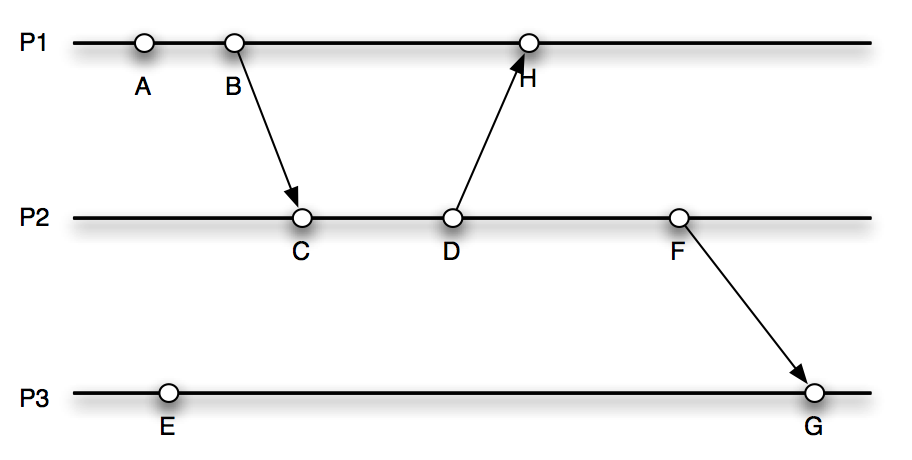
\includegraphics[width=0.5\textwidth]{Clocks.png}
\end{center}\end{figure*}

\begin{enumerate}
	\item Identify pairs of events that are logically concurrent. (In other words, in the absence of a global clock and tight time synchronization, which events cannot be distinguished as having occurred at different times?)
	\item Specify Lamport logical timestamps and vector clock timestamps for each event.
\end{enumerate}


% \item (It's party time!) You studied hard for your algorithms course, and to celebrate, you decided to throw a party for all VSP 2019 students. Some students, however, are not on good terms with others. You have a list of all $n$ students, along with information about whether any two students are not on good terms (conflicting). You would like to maximize the fun at the party, so you would like to minimize the number of pairwise conflicting students who are attending the party (no awkward encounters, please!) More precisely, you want to figure out the maximum number of students who are \emph{not} conflicting (pairwise), and, toward that end, you create a graph where each node represents a student, and an edge exists between two nodes iff the two corresponding students are not on good terms. 

% Your numerous attempts at coming up with a polynomial-time algorithm to solve this problem were not fruitful, so---because you are so eager to apply what you learned in class---you ignore organizing the party altogether and you set out to prove that this problem is $\textbf{NP}$-Complete.   

%   \begin{enumerate}
%   \item Let $\texttt{PARTY} \subset \{0,1\}^{*}$ denote the language corresponding to your problem. Write down \texttt{PARTY} precisely in terms of the graph abstraction described above. Note that we are concerned here with the \emph{decision} version of the problem: A problem whose possible answers are either \texttt{yes} or \texttt{no}. \\

% \textbf{Solution.}
% \begin{align*}
%   \texttt{PARTY} = \bigl\{ \langle  G,k \rangle: \text{graph } G \text{ has at least } k \text{ pairwise non-adjacent vertices}  \bigr \}.
% \end{align*}

% \item Show that $\texttt{PARTY} \in \textbf{NP}$. Describe both the certificate and the verifier program carefully. \\

% Recall the definition of the complexity class $\textbf{NP}$: A language $L \subseteq \{0,1\}^{*}$ is in $\textbf{NP}$ if there exists a polynomial $p:\mathbb{N} \to \mathbb{N}$ and a polynomial-time program (Turing machine) $M$ such that for every $x \in \{0, 1\}^{*}$,
% \begin{align*}
% x \in L \Longleftrightarrow \exists u \in \{0,1\}^{p(|x|) } \text{ s.t. } M(x,u) = \texttt{yes}.
% \end{align*}

% If $x \in L$ and $u \in \{0,1\}^{p(|x|)}$ satisfy $M (x,u ) = \texttt{yes}$, then we call $u$ a \emph{certificate} for $x$ (with respect to the language $L$ and machine $M$). Program $M$ is the \emph{verifier}. \\

% \textbf{Solution.} The certificate is a set of vertices $S \subset V$. Thus the size of the certificate is polynomial (at most linear) in the size of $\langle G, k \rangle$. The verifier program $M$ takes as input $G$, $k$, and a subset of vertices $S$, and returns ``yes'' if both (1) $|S| \geq k$, and (2) there is no edge in $G$ between any two vertices in $S$. Otherwise $M$ returns ``no''. In the worst case, $M$ will have to examine every pair of vertices in $S$, so, for instance, using the adjacency matrix representation, the verification of (2) takes $O(|S|^{2})$ in the worst-case, which is at most $O(|V|^{2})$.   

% \item To finish off the $\mathbf{NP}$-Completeness proof, you need to show that \texttt{PARTY} is $\textbf{NP}$-Hard. Recall that a language $L'$ is $\textbf{NP}$-Hard if every language $L$ in $\mathbf{NP}$ is polynomial-time reducible to it. Language $L \subset \{0,1\}^{*}$ is \textbf{reducible} to $L' \subset \{0,1\}^{*}$ if there exists a polynomial-time computable function $f: \{0,1\}^{*} \to \{0,1\}^{*}$ such that $x \in L$ iff $f(x) \in L'$ (denoted $L \leq_{p} L')$. We showed in class that reductions are transitive (i.e., if $L_{1} \leq_{p} L_{2}$ and $L_{2} \leq_{p} L_{3}$, then $L_{1} \leq_{p} L_{3}$), so it is sufficient to pick one language that is known to be $\mathbf{NP}$-Complete and establish a reduction from it to our problem. We mentioned in class that the language \texttt{SAT} consisting of satisfiable Boolean formulae was the first language to be shown $\mathbf{NP}$-Complete (the Cook-Levin Theorem). Let $\varphi \equiv \varphi(x_{1}, \dotsc, x_{n})$ denote a Boolean formula on $n$ Boolean variables. An example is $\varphi = (x_{1}\vee x_{2} \vee \wbar{x}_{3})\wedge (x_{2} \vee x_{3})$, with 3 variables $x_{1}, x_{2}$, and $x_{3}$. A \textbf{satisfying assignment} for $\varphi$ is $x_{1}x_{2}x_{3}=101$. Formally,
%   \begin{align*}
%     \texttt{SAT} = \bigl\{\varphi: \varphi \text{ has a satisfying assignment} \bigr\}.
%   \end{align*}

% Define a \textbf{literal} to be either $x_{i}$ or $\wbar{x}_{i}$. A Boolean formula is in 3-Normal Conjunctive Form (3-CNF) if it is the conjunction (logical and) of clauses, each of which consisting of exactly 3 literals. An example of a Boolean formula in 3-CNF is $(x_{1}\vee x_{2} \vee \wbar{x}_{3})\wedge (x_{2} \vee x_{3} \vee \wbar{x}_{4})\wedge (x_{5} \vee \wbar{x}_{6} \vee \wbar{x}_{7}) \wedge (\wbar{x}_{5} \vee \wbar{x}_{8} \vee x_{9}) $; this formula has $4$ clauses (the expression in parenthesis), and each clause is the disjunction of exactly 3 literals. Define the language  
% \begin{align*}
%     \texttt{3SAT} = \bigl \{\varphi: \varphi \text{ is a satisfiable Boolean formula in 3-CNF} \bigr \}.
%   \end{align*}
% Convince yourself, but not the grader, that every Boolean formula can be converted to an equivalent 3-CNF formula in polynomial-time, and thus \texttt{3SAT} is \textbf{NP}-Complete. 


% We wish to show that $\texttt{3SAT} \leq_{p} \texttt{PARTY}$. Finding a satisfying assignment for a 3-CNF formula may be viewed as picking exactly one literal from each clause. However, the literals should be \textbf{consistent}, in the sense that the set of literals that you obtain after picking one from each clause should not contain a variable and its negation. For instance, in $(x_{1}\vee x_{2} \vee \wbar{x}_{3})\wedge (x_{2} \vee x_{3} \vee \wbar{x}_{4})\wedge (x_{5} \vee \wbar{x}_{6} \vee \wbar{x}_{7}) \wedge (\wbar{x}_{5} \vee \wbar{x}_{8} \vee x_{9})$, the set $\{x_{1}, x_{2}, \wbar{x}_{5}, \wbar{x}_{8}\}$ is consistent, and the corresponding assignment $x_{1}x_{2}x_{5} x_{8} = 1100$ (with any truth values assigned arbitrarily to any of the other variables) gives a satisfying assignment for this formula. The set $\{x_{1}, x_{2}, x_{5}, \wbar{x}_{5}\}$, on the other hand, is not consistent. Using this observation, for a given Boolean formula $\varphi$ consisting of $m$ clauses, construct a graph $G=(V, E)$ where each node is a literal that appears in $\varphi$ (if a literal appears in more than one clause, then it has a separate node in $G$ for each such occurrence) . An edge exists between two nodes in the graph if the corresponding literals are in the same clause in $\varphi$. Note that this edge forces all the literals in one clause to be in a separate connected component. However, the constraint that the literals you choose are consistent is not yet enforced in graph $G$. \emph{You are asked to complete the construction of graph $G$ by adding more edges to enforce the consistency constraint. After you are done, given a 3-CNF Boolean formula $\varphi = \varphi(x_{1}, \dotsc, x_{n})$ with $n$ variables and $m$ clauses, show that $\varphi \in \texttt{3SAT}$ if and only if graph $G$ that you constructed has at least $m$ students who are pairwise non-conflicting (on good terms). Argue that the transformation takes time that is polynomial in both the number of variables $n$ and the number of clauses $m$ of $\varphi$. Conclude that \texttt{PARTY} is \textbf{NP}-Complete.}\\

% \textbf{Solution.} The graph construction will be complete when we connect every literal $x_{i}$ in $G$ with its negation $\wbar{x}_{i}$ by an edge. 
% \begin{itemize}
% \item Suppose that $\varphi \in \texttt{3SAT}$; i.e., $\varphi(x_{1}, \dotsc, x_{n})$ is in 3-CNF and has a satisfying assignment. Then at least one literal in each of the $m$ clauses can be assigned 1, and none of these $m$ literals are conflicting (i.e., this set of literals does not contain a variable and its negation). Denote those literals as $y_{1}, \dotsc, y_{m}$. Construct the instance $\langle G, m\rangle$. By our construction of $G$, each $y_{i}$ is in different triangles, and no $y_{i}$ and $y_{j}$ in different triangles in $G$ have an edge between them. Thus the subset of vertices in $G$ corresponding to $y_{1}, \dotsc, y_{m}$ are pairwise non-adjacent.
% \item Suppose that $f(\varphi) = \langle G, m \rangle \in \texttt{PARTY}$; i.e., graph $G$ has a subset of vertices $S$ with $|S| \geq m$, and no two vertices in $S$ have an edge between them in $G$. We want to show that we can in this case contruct a feasible assignment for $\varphi$. Indeed, by construction of $G$, every node in $S$ represents one literal from each clause in $\varphi$, and no two nodes in $S$ represent a variable and its negation in $\varphi$, so a satisfying assignment for $\varphi$ may be constructed by simply setting to 1 every literal corresponding to every node in $S$.      
% \end{itemize}

% \textbf{Note:} The abstract version of problem \texttt{PARTY} is a well-known \textbf{NP}-Complete problem called the \textbf{maximum independent set.} We saw a special case in class when we discussed the problem of selecting non-adjacent bottles in a given ordered set of bottles with different volumes to maximize the total volume you drink. We showed that a polynomial-time, dynamic programming-based solution exists, and thus this problem is in \textbf{P}. The non-adjacent bottle constraint corresponds to the nodes being independent in the solution (i.e., there is no edge between them). The non-adjacent bottle problem is a special case of the maximum independent set problem when the graph is a line (a path), and is called the \textbf{maximum independent set on a line}. The moral is that some problems are computationally intractable for general inputs, but become polynomial-time solvable for special cases of the input. Another example is the \texttt{2SAT} problem, where the boolean formula is in 2-CNF; i.e., the conjunction of clauses, each of which is the disjunction of 2 variables. \texttt{2SAT} is known to have a polynomial-time algorithm to decide it.

% \end{enumerate}

\end{enumerate}



%%%%%%%%%%%%%%%%%%%%%%%%%%%%%%%%%%%%%%%%%%%%%%%%%%%%%%%%%%%%%%%%%%%%%%%%%
%% the bibliography starts here.

%\newpage
%\bibliographystyle{acm}
%\setlength{\baselineskip}{0.8\baselineskip}
%\bibliography{../../Bibliography/CompleteBibliography}

%%%%%%%%%%%%%%%%%%%%%%%%%%%%%%%%%%%%%%%%%%%%%%%%%%%%%%%%%%%%%%%%%%%%%%%%%
%% other closing material

% \appendix
% \input{appendix.tex}

\end{document}
%%% Local Variables:
%%% mode: latex
%%% TeX-master: t
%%% End:
